% IMPORTANT: PLEASE USE XeLaTeX FOR TYPESETTING
\documentclass[10pt]{beamer}

\usetheme{Darmstadt}%{default}
\usecolortheme{beaver}
\usepackage[T1]{fontenc} 
\usepackage[utf8]{inputenc}
\usepackage[french]{babel}
\usefonttheme{serif}
\usepackage{lmodern}
\usepackage{tcolorbox}
 % pour un pdf lisible à l'écran
 % il y a d'autres choix possibles 
\usepackage{pslatex}
% \usepackage{ctex, hyperref}
\usepackage{latexsym,amsmath,xcolor,multicol,booktabs,calligra}
\usepackage{graphicx,pstricks,listings,stackengine}
\usepackage{chemfig}

\usepackage{tabularx}
% meta-data

\author{Gabriel Le Doudic}
\institute{Préparation à l'agrégation de Rennes}
% \titlebackground{images/background}

\definecolor{aquamarine}{rgb}{0.5, 1.0, 0.83}
\definecolor{applegreen}{rgb}{0.55, 0.71, 0.0}	
\definecolor{cobalt}{rgb}{0.0, 0.28, 0.67}

\definecolor{definitionf}{RGB}{220,252,220}
\definecolor{definitionl}{RGB}{39,123,69}
\definecolor{definitiono}{RGB}{72,148,101}

\definecolor{propositionf}{RGB}{255,216,218}
\definecolor{propositionl}{RGB}{38,38,38}
\definecolor{propositiono}{RGB}{109,109,109}

\definecolor{theof}{RGB}{255,216,218}
\definecolor{theol}{RGB}{160,0,4}
\definecolor{theoo}{RGB}{221,65,100}

\definecolor{avertl}{RGB}{163,92,0}
\definecolor{averto}{RGB}{255,144,0}

\definecolor{histf}{RGB}{241,238,193}

\definecolor{metf}{RGB}{220,230,240}
\definecolor{metl}{RGB}{56,110,165}
\definecolor{meto}{RGB}{109,109,109}


\definecolor{remf}{RGB}{230,240,250}
\definecolor{remo}{RGB}{150,150,150}

\definecolor{exef}{RGB}{240,240,240}

\definecolor{protf}{RGB}{247,228,255}
\definecolor{protl}{RGB}{105,0,203}
\definecolor{proto}{RGB}{174,88,255}

\definecolor{grid}{RGB}{180,180,180}

\definecolor{titref}{RGB}{230,230,230}

\definecolor{vert}{RGB}{23,200,23}

\definecolor{violet}{RGB}{180,0,200}

\definecolor{copper}{RGB}{217, 144, 88}
%% CADRES

\newtcolorbox{defi}[1]{
	colback=applegreen!5!white,
  	colframe=applegreen!65!black,
	fonttitle=\bfseries,
  	title={#1}}
\newtcolorbox{Programme}[1]{
	colback=cobalt!5!white,
  	colframe=cobalt!65!black,
	fonttitle=\bfseries,
  	title={#1}}  
\newtcolorbox{Resultat}[1]{
	colback=theof,%!5!white,
	colframe=theoo!85!black,
  fonttitle=\bfseries,
	title={#1}} 
\usepackage{tikz}
\usepackage{array}
\usepackage[scientific-notation=true]{siunitx}
\usetikzlibrary{matrix}
\newcommand{\diff}{\mathrm{d}}
% document body
\begin{document}
\begin{frame}{}
    \titlepage

    \begin{tabularx}{\textwidth}{l@{:\,\,}X}
        \textbf{Niveau} 	  &	Deuxième année de CPGE\\
        \textbf{Prérequis} & Physique ondulatoire\\
        &			Notion de fonction d'onde, équation de Schrödinger, cas d'une particule libre\\
        & 			Puits carré de potentiel de profondeur infinie et finie, courant de probabilité
    \end{tabularx}
\end{frame}
% \maketitle
% --------- Sommaire ---------
% \begin{frame}
%     \tableofcontents
% \end{frame}      
% ----------------------------

\section{Barrière de potentiel}
\subsection{Fonction d'onde propre}
\subsection{Probabilité de réflexion et de transmission. Effet tunnel}

\begin{frame}{Réflexion et transmission}
    Conditions aux limites:	
			\vspace{-.35cm}
			\begin{multicols}{2}
				\noindent
				\begin{align}
					A_1+B_1&=A_2+B_2 \label{1}\\
					\imath k(A_1-B_1)&=q(A_2-B_2)\label{2}
				\end{align}
				\begin{align}
					A_2e^{qa}+B_2e^{-qa}&=A_3e^{\imath ka}\label{3}\\
					q(A_2e^{qa}-B_2e^{-qa})&=\imath kA_3e^{\imath ka}\label{4}
				\end{align}
			\end{multicols}
            Résolution du système pour trouver une relation directe entre $A_1$ et $A_3$:
			\begin{itemize}
				\item[$\bullet$] $\eqref{3}+\frac{1}{q}\eqref{4}$ donne $A_2=f(A_3)$
				\item[$\bullet$]  $\eqref{3}-\frac{1}{q}\eqref{4}$ donne $B_2=f(A_3)$
				\item[$\bullet$] on peut alors exprimer $A_2+B_2$ et $A_2-B_2$ en fonction de $A_3$
				\item[$\bullet$] enfin $\eqref{1}+\frac{1}{\imath k}\eqref{2}$ donne $2A_1=A_2+B_2-\imath\frac{q}{k}(A_2-B_2)$.
			\end{itemize}
			À partir de là, on a une expression de $A_1$ en fonction de $A_3$.
			
			\vspace{.5cm}
			\pause
			D'où le coefficient de transmission:
			\begin{equation*}
				T=\frac{1}{1+\frac{\left(k^2+q^2\right)^2}{4q^2k^2}\mathrm{sh}^2(qa)}
			\end{equation*}
\end{frame}
\subsection{Approximation de barrière épaisse}

\begin{frame}{\insertsubsection}
    Quelques ordres de grandeur (d'après \textit{J'intègre, PC}):
    \medskip

    \begin{tabular}{lccccc}
        Particule	&	$m$ (kg)	& $V_0$ (eV)	& $a$ (nm)	&	$\delta$ (nm)	&	$T$\\\hline\hline
        Électron	&	\num{1e-30}	& 4		&	\num{0,3}	&	\num{0,1}	&	\num{1e-2}\\
        Électron	&	\num{1e-30}	& 40	&	\num{0,3}	&	\num{4e-2}	&	\num{1e-6}\\
        Électron	&	\num{1e-30}	& 4		&	\num{3}		&	\num{0,1}	&	\num{1e-20}\\
        Proton		&	\num{1e-27}	& 4		&	\num{0,3}	&	\num{4e-3}	&	\num{1e-63}\\
        Proton		&	\num{1e-27}	& 4		&	\num{3}	&	\num{2e-3}	&	\num{1e-628}\\\hline
    \end{tabular}
\end{frame}

\section{Radioactivité $\alpha$}

\subsection{Description et résultats expérimentaux}

\begin{frame}{\insertsubsection}
    \begin{figure}
        \centering
        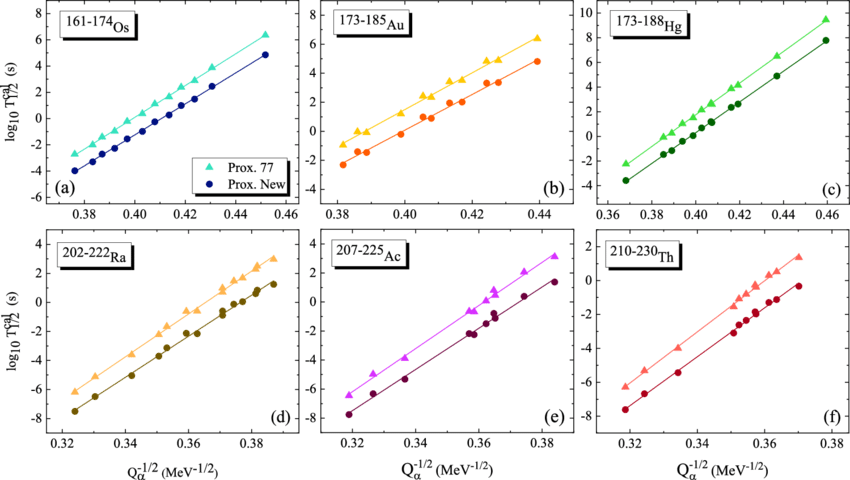
\includegraphics[width=.8\linewidth]{Geiger-Nuttall.png}
        \caption{\scriptsize \textit{Gharaei, Reza \& Mohammadi, Sara. (2019). (doi:10.1140/epja/i2019-12804-5)}}
    \end{figure}
    \begin{center}
        \begin{tabular}{ccc}
            Noyau & Temps de demi--vie (s) & $E$ (MeV)\\\hline
            $^{222}_{86}\mathrm{Ra}$ & \num{3.3e5} & \num{5.6}\\
            $^{226}_{86}\mathrm{Ra}$ & \num{5.4e10} & \num{4.9}\\
            $^{232}_{90}\mathrm{Th}$ & \num{4.4e17} & \num{4.0}
        \end{tabular}
    \end{center}
\end{frame}


\subsection{Théorie de la radioactivité $\alpha$}

\begin{frame}{Calcul du coefficient de transmission}
    \begin{equation}
        \ln T = - \dfrac{2\sqrt{2m}}{\hbar}\sqrt{\dfrac{2e^2Z^\prime}{4\pi\epsilon_0}}\dfrac{1}{\sqrt{R_c}}\int_R^{R_c}\sqrt{\dfrac{R_c}{R}-1}\diff r
    \end{equation}

On admet alors le résultat suivant:
    \begin{equation*}
        \int_{x_0}^{x_m}\sqrt{\frac{x_m}{x}-1}dx\simeq x_m\left(\frac{\pi}{2}-2\sqrt{\frac{x_0}{x_m}}\right)
    \end{equation*}
Après quelques lignes de calcul, on obtient: $\ln T = a - \dfrac{b}{\sqrt{E}}$, avec:
\begin{align*}
    a&=\frac{4e}{\hbar}\sqrt{\frac{mZ'r_0}{\pi\varepsilon_0}}A^{1/6}\\
    b&=\frac{{\rm e}^2Z'}{2\hbar\varepsilon_0}\sqrt{2m}
\end{align*}
\end{frame}

\subsection{Comparaison avec les données expérimentales}
\begin{frame}{\insertsubsection}
    \begin{figure}
        \centering
        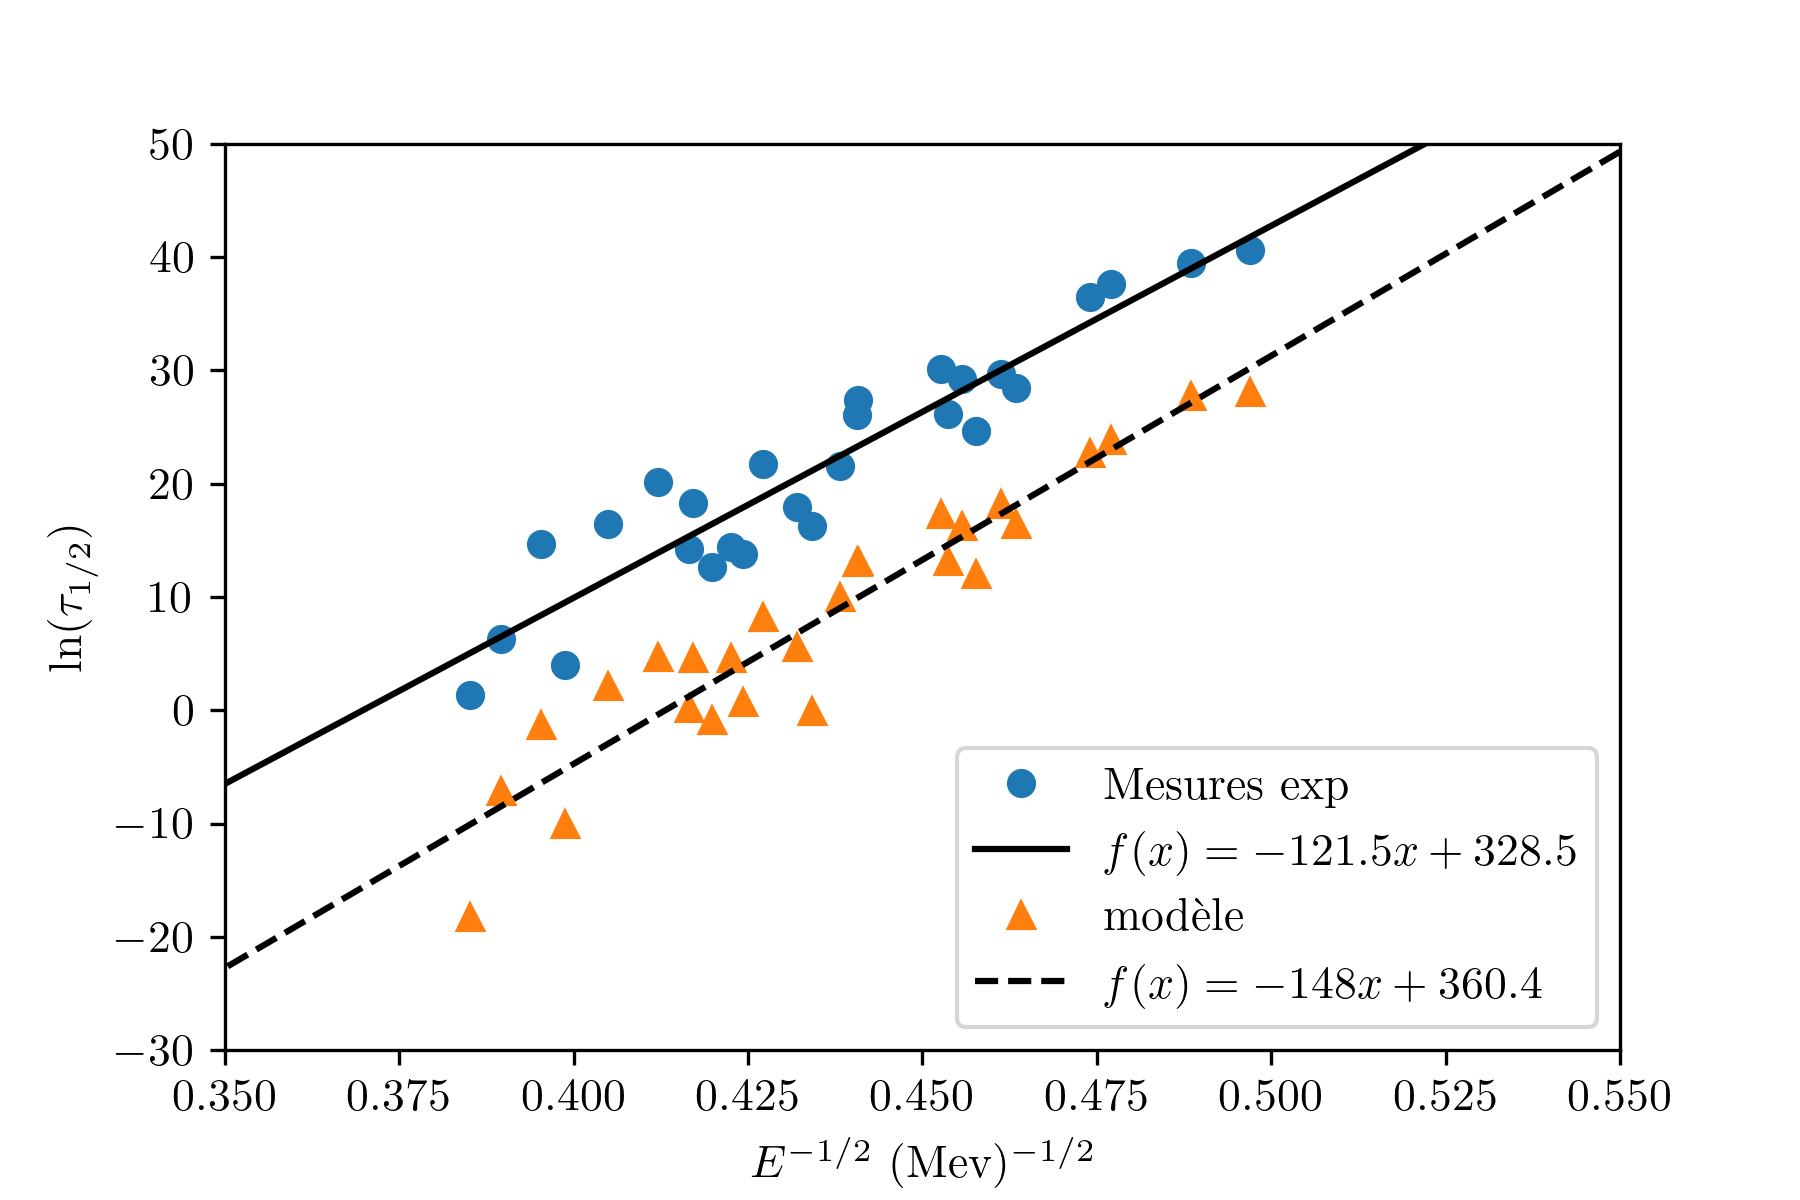
\includegraphics[width=1\textwidth]{Radioactivite_alpha.png}
    \end{figure}
\end{frame}

\begin{frame}{\insertsubsection}
    \begin{figure}
        \centering
        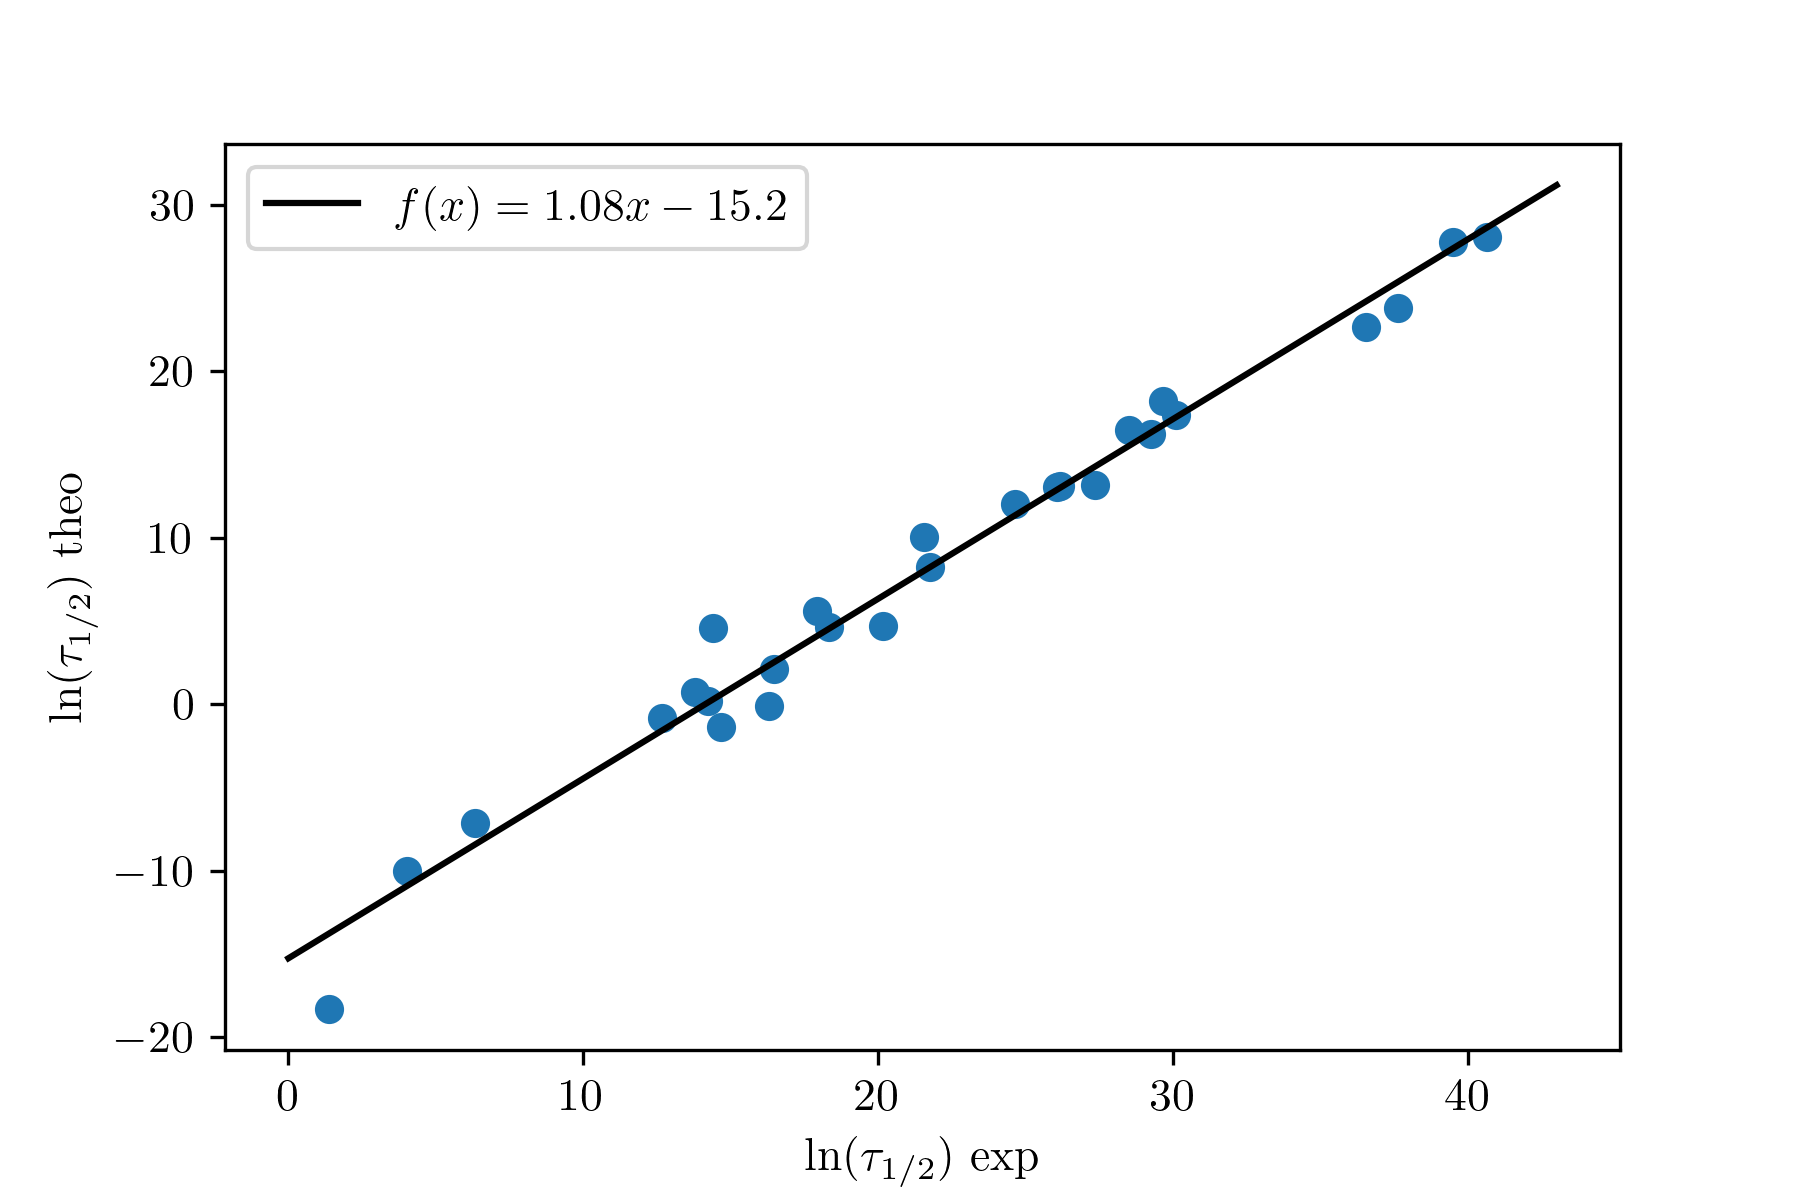
\includegraphics[width=1\textwidth]{Modele_vs_exp.png}
    \end{figure}
\end{frame}


\end{document}